\chapter{Element Parameter Groups}
\label{c:ele.groups}

Generally, element parameters are grouped into ``\vn{element} \vn{parameter} \vn{group}'' 
types which is discussed in \sref{c:ele}.

Element parameter groups inherit from the abstract type \vn{EleParameterGroup} which
in turn inherits from \vn{BaseEleParameterGroup}. Some
parameter groups have sub-group components. 
These sub-groups also inherit from \vn{BaseEleParameterGroup}:
\begin{example}
  abstract type BaseEleParameterGroup end
  abstract type EleParameterGroup <: BaseEleParameterGroup end
  abstract type EleParameterSubGroup <: BaseEleParameterGroup end
\end{example}

Notes:
\begin{itemize}
%
\item
All parameter groups have associated docstrings that can be accessed using the REPL help system.
%
\item
NaN denotes parameter that is not set.
%
\item
Parameters marked ``dependent'' are parameters calculated by \accellat and not settable by the User.
%
\end{itemize}


The parmeters groups are:
\begin{table}[htb]
\centering
{\tt
\begin{tabular}{llll} \toprule
  {\it Group}        & {\it Section}             & {\it Group}         & {\it Section}         \\ \midrule
 AlignmentGroup      & \sref{s:align.g}          & LordSlaveGroup      & \sref{s:lord.slave.g} \\
 ApertureGroup       & \sref{s:aperture.g}       & MasterGroup         & \sref{s:master.g}     \\
 BMultipoleGroup     & \sref{s:bmultipole.g}     & PatchGroup          & \sref{s:patch.g}      \\ 
 BeamBeamGroup       & \sref{s:beam.beam.g}      & RFCommonGroup       & \sref{s:rfcommon.g}   \\
 BendGroup           & \sref{s:bend.g}           & RFCavityGroup       & \sref{s:rfcavity.g}    \\ 
 EMultipoleGroup     & \sref{s:emultipole.g}     & RFAutoGroup         & \sref{s:rfauto.g}   \\
 FloorPositionGroup  & \sref{s:floor.pos.g}      & ReferenceGroup      & \sref{s:reference.g}  \\
 GirderGroup         & \sref{s:girder.g}         & SolenoidGroup       & \sref{s:solenoid.g}   \\
 InitParticleGroup   & \sref{s:init.particle.g}  & StringGroup         & \sref{s:string.g}     \\
 LCavityGroup        & \sref{s:lcavity.g}        & TrackingGroup       & \sref{s:tracking.g}   \\
 LengthGroup         & \sref{s:length.g}         & TwissGroup          & \sref{s:twiss.g}      \\ 
  \bottomrule
\end{tabular}
} 
\caption{Table of element parameter groups.}
\label{t:particle.groups}
\end{table}

%---------------------------------------------------------------------------------------------------
\section{AlignmentGroup}
\label{s:align.g}

\begin{figure}
\centering 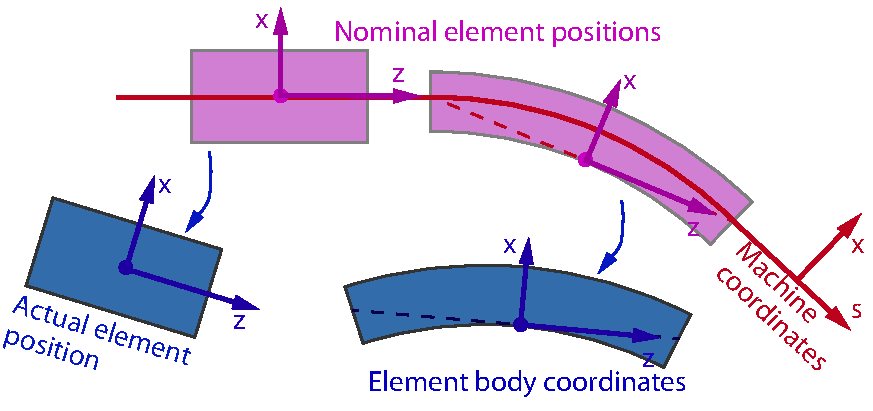
\includegraphics{alignment-ref.pdf} 
\caption[Element alignment.]  
{AlignmentGroup parameters The reference point is the origin
about which the element alignment is calculated. 
A) For straight elements, the reference point is in the center of the element. 
For \vn{Bend} elements, the reference point is at the midpoint of the chord connecting
the entrance point to the exit point. The drawing for the bend is valid for a \vn{ref_tilt}
of zero. For non-zero \vn{ref_tilt}, the outward direction from the bend center will not be
the $x$-axis. 
}  \label{f:alignment}
\end{figure}

\begin{figure}
\centering 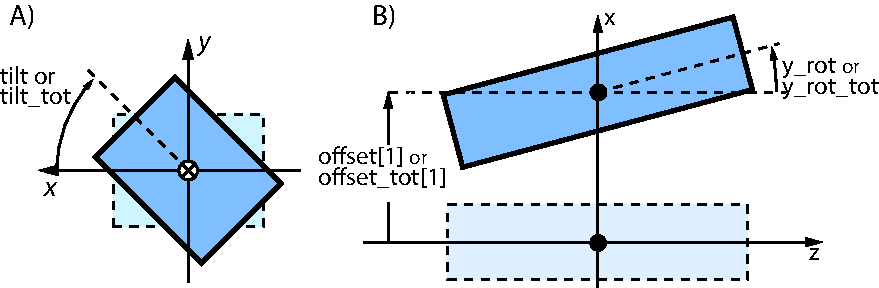
\includegraphics{alignment2.pdf} \caption[Alignment geometry.]  
{Alignment geometry. A) \vn{tilt} (or \vn{tilt_tot}) rotation. B) Combined
\vn{offset[1]} with \vn{y_rot} (or \vn{offset_tot[1]} with \vn{y_rot_tot}).
}  \label{f:alignment}
\end{figure}

The alignment group gives the alignment (position and angular orientation) of the physical element 
relative to the nominal position defined by the machine coordinates (\sref{s:orient}).
Alignment is specified with respect to the ``alignment reference point'' of an element as shown
in Fig~\ref{s:alignment}. The \vn{Bend} reference point is chosen to be the center of the chord
connecting the two ends. 
This reference point was chosen over using the midpoint on the reference orbit arc since a 
common simulation problem is to simulate a bend with a \vn{tilt} keeping the entrance and exit
endpoints fixed.

The parameters of the \vn{AlignmentGroup} can be divided into two sub-groups. 
One group has a \vn{_tot} suffix:
\begin{example}
  offset_tot::Vector - $[x, y, z]$ offset.
  x_rot_tot::Number  - Rotation around the x-axis.
  y_rot_tot::Number  - Rotation around the z-axis.
  tilt_tot::Number   - Rotation around the z-axis. 
\end{example}
These ``total alignment'' parameters give the alignment of the element with 
with respect to the machine coordinates.
The other sub-group of parameters do not have a \vn{_tot} suffix:
\begin{example}
  offset::Vector - $[x, y, z]$ offset.
  x_rot::Number  - Rotation around the x-axis.
  y_rot::Number  - Rotation around the z-axis.
  tilt::Number   - Rotation around the z-axis. 
\end{example}
These ``relative alignment'' parameters give the alignment of the element with respect 
to any \vn{Girder} that is supporting the element. 
If there is no support \vn{Girder}, the total alignment will be the same as the relative
alignment. The relative alignment can be set by the User. 
The total alignment is computed by \accellat based upon the relative alignment and the alignment
of any \vn{Girder}. \vn{Girder} elements themselves also have both relative and total
alignments since Girders can support other Girders.


%---------------------------------------------------------------------------------------------------
\section{ApertureGroup}
\label{s:aperture.g}


%---------------------------------------------------------------------------------------------------
\section{BMultipoleGroup}
\label{s:bmultipole.g}

%---------------------------------------------------------------------------------------------------
\section{BeamBeamGroup}
\label{s:beam.beam.g}

%---------------------------------------------------------------------------------------------------
\section{BendGroup}
\label{s:bend.g}

%---------------------------------------------------------------------------------------------------
\section{EMultipoleGroup}
\label{s:emulitipole.g}

%---------------------------------------------------------------------------------------------------
\section{FloorPositionGroup}
\label{s:floor.pos.g}

%---------------------------------------------------------------------------------------------------
\section{GirderGroup}
\label{s:girder.g}

%---------------------------------------------------------------------------------------------------
\section{InitParticleGroup}
\label{s:init.particle.g}

%---------------------------------------------------------------------------------------------------
\section{LCavityGroup}
\label{s:lcavity.g}

%---------------------------------------------------------------------------------------------------
\section{LengthGroup}
\label{s:length.g}

%---------------------------------------------------------------------------------------------------
\section{LordSlaveGroup}
\label{s:lord.slave.g}

%---------------------------------------------------------------------------------------------------
\section{MasterGroup}
\label{s:master.g}

%---------------------------------------------------------------------------------------------------
\section{PatchGroup}
\label{s:patch.g}

%---------------------------------------------------------------------------------------------------
\section{RFCommonGroup}
\label{s:rfcommon.g}

%---------------------------------------------------------------------------------------------------
\section{RFCavityGroup}
\label{s:rfcavity.g}

%---------------------------------------------------------------------------------------------------
\section{RFAutoGroup}
\label{s:rfauto.g}

%---------------------------------------------------------------------------------------------------
\section{ReferenceGroup}
\label{s:reference.g}

%---------------------------------------------------------------------------------------------------
\section{SolenoidGroup}
\label{s:solenoid.g}

%---------------------------------------------------------------------------------------------------
\section{StringGroup}
\label{s:string.g}

%---------------------------------------------------------------------------------------------------
\section{TrackingGroup}
\label{s:tracking.g}

%---------------------------------------------------------------------------------------------------
\section{TwissGroup}
\label{s:twiss.g}

